\documentclass[11pt]{article}
\usepackage{tcolorbox}
\usepackage{textcomp}
\usepackage[os=win]{menukeys}
\usepackage{pdflscape}
\usepackage{rotating}
\usepackage{listings}

\newcommand{\numpy}{{\tt numpy}}    % tt font for numpy

\topmargin -.5in
\textheight 9in
\oddsidemargin -.25in
\evensidemargin -.25in
\textwidth 7in

\begin{document}

% ========== Edit your name here
\author{Dr. Neil Eliot / Dr. Alun Moon}
\title{KF5004\\------\\Network Design\\------\\The Implementation of a \texttt{DNS} infrastructure (\texttt{BIND9}) and Web Server Farm facilities
(\texttt{Apache, PHP, NFS, and MySQL})\\------}
\date{September 2019}
\maketitle

\newpage
\tableofcontents
\newpage

\section{Revisions}
\begin{table}[ht]
    \begin{tabular}{|p{1.5cm}|p{11cm}|p{2cm}|p{1.5cm}|} 
      \hline
      \multicolumn{1}{|c|}{Version} & \multicolumn{1}{|c|}{Description} & \multicolumn{1}{|c|}{Date}& \multicolumn{1}{|c|}{Author} \\ 
      \hline
      1.0 & Initial Schematic design. This is not a network diagram! It is indicative of the company deployment.& 03/06/2107 & NE\\
      \hline
      1.1 & Updated requirements for subdomain of staff.uun and updated configuration file structures and locations.& 01/09/2108 & NE\\
      \hline
      1.2 & Updated subdomain configuration to allow zone transfer to primary 1.& 10/12/2108 & NE\\
      \hline
    \end{tabular}
\end{table}
\newpage

\begin{landscape}
        \begin{figure}
        \begin{center}
            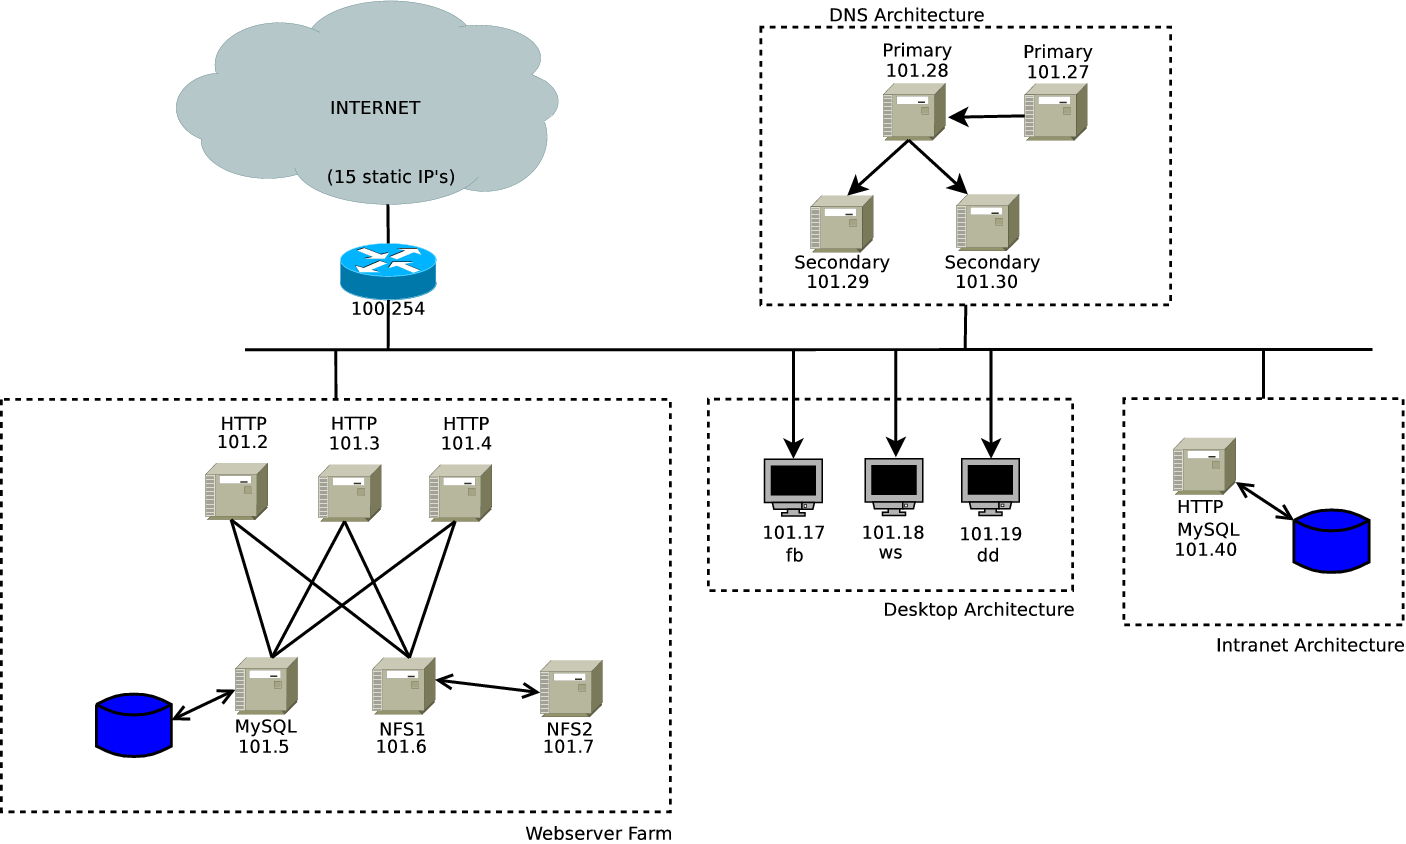
\includegraphics[width=1\linewidth]{Schematic.png}
            \caption{Schematic}
        \end{center}
      \end{figure}
\end{landscape}

\section{Primary Server 1}
\begin{table}[ht]
    \begin{tabular}{|p{17.5cm}|} 
        \hline
        \texttt{\textbf{/etc/netplan/10-cloud-init.yaml}}\\ 
        \hline
        \lstset{
                basicstyle=\scriptsize\ttfamily,
              }
              \begin{lstlisting}
# NETWORK CONFIG
network:
    version: 2
    ethernets:
      ens33:
        addresses: [192.168.101.28/16]
        gateway4: 192.168.100.254
        nameservers:
          search: [tech.co.uk, unn.co.uk]
          addresses: [8.8.8.8, 8.8.4.4]
        \end{lstlisting}\\
        \hline
    \end{tabular}
\end{table}

\begin{table}[ht]
    \begin{tabular}{|p{17.5cm}|} 
        \hline
        \texttt{\textbf{/etc/bind/named.conf.local}}\\ 
        \hline
        \lstset{
                basicstyle=\scriptsize\ttfamily,
              }
              \begin{lstlisting}
// 
// Do any local configuration here //
// Consider adding the 1918 zones here, if they are not used in your
// organization
// include "/etc/bind/zones.rfc1918";
                
zone "unn.co.uk" {
    type master;
    file "/etc/bind/db.unn.co.uk";
    allow-transfer {192.168.101.29; 192.168.101.30;};
    allow-query {192.168.101.29; 192.168.101.30;};
};
                
zone "tech.co.uk" {
    type master;
    file "/etc/bind/db.unn.co.uk";
    allow-transfer {192.168.101.29; 192.168.101.30;};
    allow-query {192.168.101.29; 192.168.101.30;};
};
                
zone "staff.unn.co.uk" {
    type slave;
    masters {192.168.101.27};
    allow-transfer {192.168.101.29; 192.168.101.30;};
    allow-query {192.168.101.29; 192.168.101.30;};
};
                
zone "168.192.in-addr.arpa" {
    type master;
    file "/etc/bind/db.168.192.in-addr.arpa";
    allow-transfer {192.168.101.29; 192.168.101.30;};
    allow-query {192.168.101.29; 192.168.101.30;};
};
        \end{lstlisting}\\
        \hline
    \end{tabular}
\end{table}

\begin{table}[ht]
    \begin{tabular}{|p{17.5cm}|} 
        \hline
        \texttt{\textbf{/etc/bind/named.conf.options}}\\ 
        \hline
        \lstset{
                basicstyle=\scriptsize\ttfamily,
              }
              \begin{lstlisting}
options {
    directory "/var/cache/bind";
            
    // If there is a firewall between you and nameservers you want
    // to talk to, you may need to fix the firewall to allow multiple
    // ports to talk.  See http://www.kb.cert.org/vuls/id/800113
            
    // If your ISP provided one or more IP addresses for stable 
    // nameservers, you probably want to use them as forwarders.  
    // Uncomment the following block, and insert the addresses replacing 
    // the all-0's placeholder.
            
    // forwarders {
    //         8.8.8.8;
    // };
            
    //========================================================================
    // If BIND logs error messages about the root key being expired,
    // you will need to update your keys.  See https://www.isc.org/bind-keys
    //========================================================================
    dnssec-validation auto;                                              
    auth-nxdomain no;    # conform to RFC1035
};
        \end{lstlisting}\\
        \hline
    \end{tabular}
\end{table}   

\begin{table}[ht]
    \begin{tabular}{|p{17.5cm}|} 
        \hline
        \texttt{\textbf{/etc/bind/db.unn.co.uk}}\\ 
        \hline
        \lstset{
                basicstyle=\scriptsize\ttfamily,
              }
              \begin{lstlisting}
$TTL    43200 
$ORIGIN unn.co.uk.
@  1d  IN  SOA ns1.unn.co.uk. hostmaster.unn.co.uk. (
                2017090807 ; sn
                172800     ; ref
                900        ; ret
                1209600    ; exp
                3600       ; nx
            )
@                           IN       NS                 ns1.unn.co.uk.
                            IN       NS                 ns2.unn.co.uk.
                            IN       MX      10         mail.microsoft.com.
                ns1         IN       A                  192.168.101.29
                ns2         IN       A                  192.168.101.30
                ns3         IN       A                  192.168.101.28
                web         IN       A                  192.168.101.40
                www         IN       A                  192.168.101.2
                            IN       A                  192.168.101.3
                            IN       A                  192.168.101.4
                ftp         IN       CNAME              web
                intranet    IN       CNAME              web
                mysql       IN       A                  192.168.101.5
                nfs1        IN       A                  192.168.101.6
                nfs2        IN       A                  192.168.101.7
        \end{lstlisting}\\
        \hline
    \end{tabular}
\end{table} 

\begin{table}[ht]
    \begin{tabular}{|p{17.5cm}|} 
        \hline
        \texttt{\textbf{/etc/bind/db.tech.co.uk}}\\ 
        \hline
        \lstset{
                basicstyle=\scriptsize\ttfamily,
              }
              \begin{lstlisting}
$TTL    0 
$ORIGIN tech.co.uk.
@  1d  IN  SOA ns1.unn.co.uk. hostmaster.unn.co.uk. (
                    2017092307 ; sn
                    1800       ; ref
                    900        ; ret
                    604800     ; exp
                    14400      ; nx
                )
@                IN        NS               ns1.unn.co.uk.
                 IN        NS               ns2.unn.co.uk.
A12345678        IN        A                192.168.101.40
web              IN        CNAME            A12345678
A12345679        IN        A                192.168.101.2
www1             IN        CNAME            A12345679
A12345680        IN        A                192.168.101.3
www2             IN        CNAME            A12345680
A12345681        IN        A                192.168.101.4
www3             IN        CNAME            A12345681
www              IN        A                192.168.101.2
                 IN        A                192.168.101.3
                 IN        A                192.168.101.4
A12345682        IN        A                192.168.101.5
mysql            IN        CNAME            A12345682
A12345683        IN        A                192.168.101.6
nfs1             IN        CNAME            A12345683
A12345684        IN        A                192.168.101.7
nfs2             IN        CNAME            A12345684
A12345685        IN        A                192.168.101.17
A12345686        IN        A                192.168.101.18
A12345687        IN        A                192.168.101.19
A12345688        IN        A                192.168.101.20
A12345689        IN        A                192.168.101.21
A12345690        IN        A                192.168.101.22
A12345691        IN        A                192.168.101.23
A12345692        IN        A                192.168.101.24
A12345693        IN        A                192.168.101.25
A12345694        IN        A                192.168.101.26
A12345695        IN        A                192.168.101.27
A12345696        IN        A                192.168.101.28
A12345697        IN        A                192.168.101.29
A12345698        IN        A                192.168.101.30
        \end{lstlisting}\\
        \hline
    \end{tabular}
\end{table}

\begin{table}[ht]
    \begin{tabular}{|p{17.5cm}|} 
        \hline
        \texttt{\textbf{/etc/bind/db.168.192.in-addr.arpa}}\\ 
        \hline
        \lstset{
                basicstyle=\scriptsize\ttfamily,
              }
              \begin{lstlisting}
$TTL 604800
$ORIGIN 168.192.in-addr.arpa.
@  1d        IN SOA        ns1.unn.co.uk. hostmaster.unn.co.uk. (
                            2015092303 ; sn
                            604800     ; ref
                            86400      ; ret
                            2419200    ; exp
                            604800     ; nx
                    )
                       NS     ns1.unn.co.uk.
                       NS     ns2.unn.co.uk.
2.101                  PTR    www.tech.co.uk.
3.101                  PTR    www.tech.co.uk.
4.101                  PTR    www.tech.co.uk.
5.101                  PTR    mysql.unn.co.uk.
        \end{lstlisting}\\
        \hline
    \end{tabular}
\end{table}

\clearpage
\section{Primary Server 2}
\begin{table}[ht]
    \begin{tabular}{|p{17.5cm}|} 
        \hline
        \texttt{\textbf{/etc/netplan/10-cloud-init.yaml}}\\ 
        \hline
        \lstset{
                basicstyle=\scriptsize\ttfamily,
              }
              \begin{lstlisting}
# NETWORK CONFIG
network:
    version: 2
    ethernets:
        ens33:
            addresses: [192.168.101.27/16]
            gateway4: 192.168.100.254
            nameservers:
                search: [tech.co.uk, unn.co.uk]
                addresses: [192.168.100.1,8.8.4.4]
        \end{lstlisting}\\
        \hline
    \end{tabular}
\end{table}

\begin{table}[ht]
    \begin{tabular}{|p{17.5cm}|} 
        \hline
        \texttt{\textbf{/etc/bind/named.conf.local}}\\ 
        \hline
        \lstset{
                basicstyle=\scriptsize\ttfamily,
              }
              \begin{lstlisting}
// 
// Do any local configuration here //
// Consider adding the 1918 zones here, if they are not used in your
// organization
// include "/etc/bind/zones.rfc1918";
                
zone "staff.unn.co.uk" {
        type master;
        file "/etc/bind/db.staff.unn.co.uk";
        allow-transfer {192.168.101.28;};
        allow-query{192.168.101.28;};
        notify no;
};
        \end{lstlisting}\\
        \hline
    \end{tabular}
\end{table}

\begin{table}[ht]
    \begin{tabular}{|p{17.5cm}|} 
        \hline
        \texttt{\textbf{/etc/bind/named.conf.options}}\\ 
        \hline
        \lstset{
                basicstyle=\scriptsize\ttfamily,
              }
              \begin{lstlisting}
options {
    directory "/var/cache/bind";
            
    // If there is a firewall between you and nameservers you want
    // to talk to, you may need to fix the firewall to allow multiple
    // ports to talk.  See http://www.kb.cert.org/vuls/id/800113
            
    // If your ISP provided one or more IP addresses for stable 
    // nameservers, you probably want to use them as forwarders.  
    // Uncomment the following block, and insert the addresses replacing 
    // the all-0's placeholder.
            
    // forwarders {
    //         8.8.8.8;
    // };
            
    //========================================================================
    // If BIND logs error messages about the root key being expired,
    // you will need to update your keys.  See https://www.isc.org/bind-keys
    //========================================================================
    dnssec-validation auto;                                              
    auth-nxdomain no;    # conform to RFC1035
};
        \end{lstlisting}\\
        \hline
    \end{tabular}
\end{table}

\begin{table}[ht]
    \begin{tabular}{|p{17.5cm}|} 
        \hline
        \texttt{\textbf{/etc/bind/db.staff.unn.co.uk}}\\ 
        \hline
        \lstset{
                basicstyle=\scriptsize\ttfamily,
              }
              \begin{lstlisting}
$TTL    43200 
$ORIGIN staff.unn.co.uk.
@  1d  IN  SOA ns1.unn.co.uk. hostmaster.unn.co.uk. (
                        2017090801 ; sn
                        172800     ; ref
                        900        ; ret
                        1209600    ; exp
                        3600       ; nx
                )
@                 IN        NS               ns1.unn.co.uk.
                  IN        NS               ns2.unn.co.uk.
ns4               IN        A                192.168.101.27
web               IN        A                192.168.101.40
fb                IN        A                192.168.101.17                                
ws                IN        A                192.168.101.18                                
dd                IN        A                192.168.101.19                                
ne                IN        A                192.168.101.20                        
ly                IN        A                192.168.101.21
        \end{lstlisting}\\
        \hline
    \end{tabular}
\end{table}

\clearpage
\section{Secondary Server 1}

\end{document}
